\documentclass[border=10pt]{standalone}

\usepackage{tikz}
\usepackage{tikzsymbols}
\usetikzlibrary{calc,patterns,shapes.geometric}

\def\centerarc[#1](#2)(#3:#4:#5){\draw[#1] ($(#2)+({#5*cos(#3)},{#5*sin(#3)})$) arc (#3:#4:#5);}

\begin{document}
	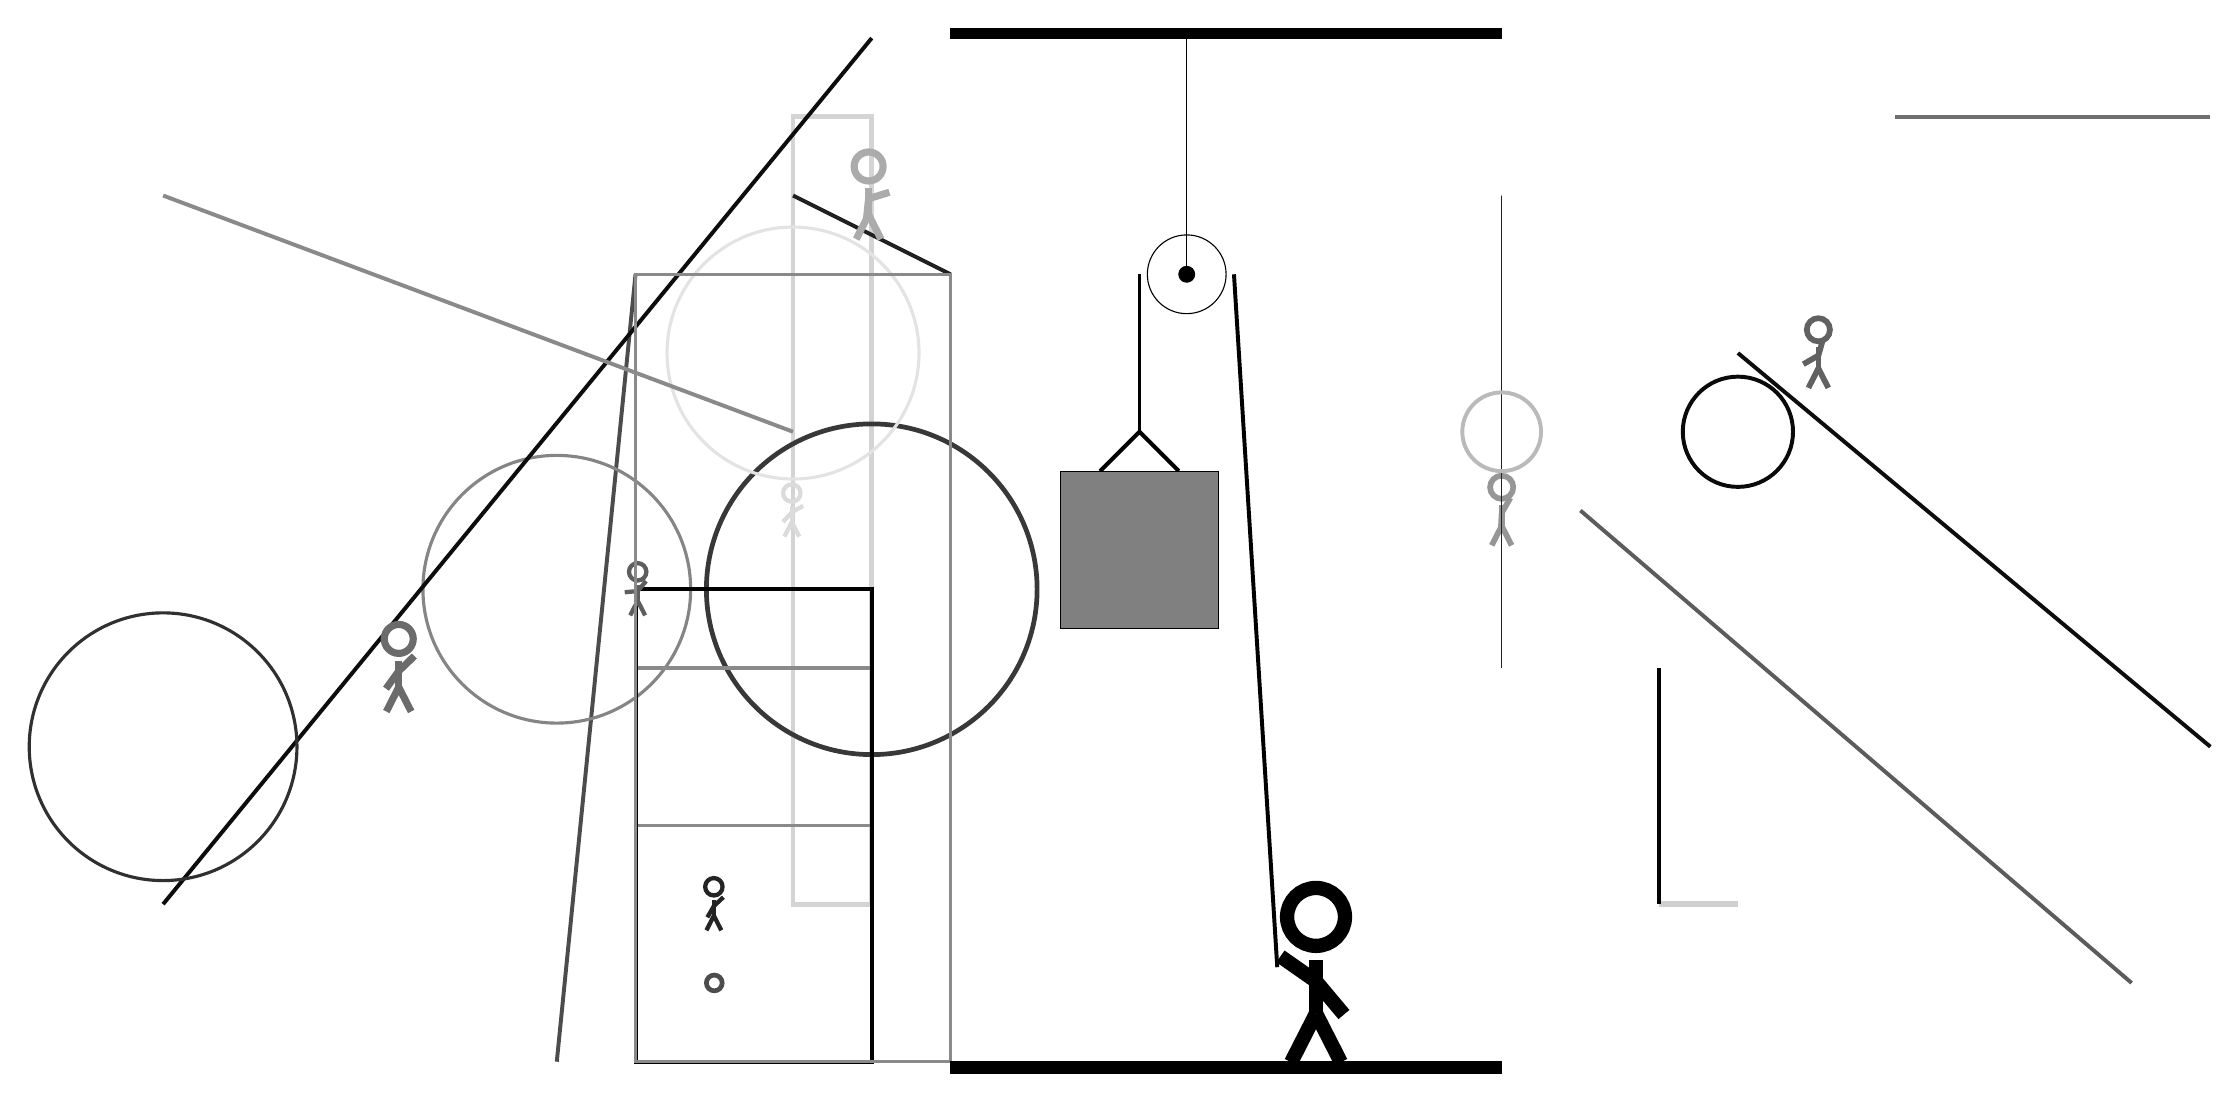
\begin{tikzpicture}
		%%%%% START %%%%%
		
		\draw[fill=black] (-2, 10) rectangle (5, 10.125);
		
		\draw (1, 7) circle (0.5);
		\draw[fill=black] (1, 7) circle (0.1);
		\draw (1, 10) -- (1, 7);
		
		\draw[line width=0.5mm, color=black!70](-7, -3) -- (-6, 7);
		
		\draw [line width=0.4mm, color=black!48](-7, 3) circle (1.7);
		\draw[line width=0.6mm, color=black!17] (-4, -1) rectangle (-3, 9);
		\node[line width=0.7mm, color=black!62] at (9, 6) {\Strichmaxerl[4][30][74]};
		\draw[line width=0.5mm, color=black!95](-3, 10) -- (-12, -1);
		\draw [line width=0.6mm, color=black!78](-3, 3) circle (2.1);
		
		\draw [line width=0.4mm, color=black!11](-4, 6) circle (1.6);
		
		\draw[line width=0.5mm, color=black!95](8, 6) -- (14, 1);
		\draw[line width=0.5mm, color=black!46](-4, 5) -- (-12, 8);
		\draw[line width=0.7mm, color=black!19] (7, -1) rectangle (8, -1);
		\node[line width=0.3mm, color=black!86] at (-5, -1) {\Strichmaxerl[3][60][43]};
		
		\node[line width=0.5mm, color=black!41] at (5, 4) {\Strichmaxerl[4][87][60]};
		\draw[line width=0.5mm, color=black!46] (-3, 2) rectangle (-6, 0);
		
		\draw [line width=0.6mm, color=black!70](-5, -2) circle (0.1);
		\draw[line width=0.2mm, color=black!87] (5, 8) rectangle (5, 2);
		\draw[line width=0.5mm, color=black!100] (-3, 3) rectangle (-6, -3);
		
		\node[line width=0.5mm, color=black!63] at (-6, 3) {\Strichmaxerl[3][5][50]};
		\draw [line width=0.5mm, color=black!27](5, 5) circle (0.5);
		\draw [line width=0.4mm, color=black!81](-12, 1) circle (1.7);
		\draw[line width=0.5mm, color=black!99](7, 2) -- (7, -1);
		\draw[line width=0.5mm, color=black!87](-2, 7) -- (-4, 8);
		\node[line width=0.7mm, color=black!58] at (-9, 2) {\Strichmaxerl[5][54][44]};
		
		\draw [line width=0.5mm, color=black!96](8, 5) circle (0.7);
		\node[line width=0.5mm, color=black!14] at (-4, 4) {\Strichmaxerl[3][47][30]};
		\draw[line width=0.5mm, color=black!64](6, 4) -- (13, -2);
		\draw[line width=0.4mm, color=black!46] (-2, -3) rectangle (-6, 7);
		
		\node[line width=0.3mm, color=black!33] at (-3, 8) {\Strichmaxerl[5][84][17]};
		\draw[line width=0.5mm, color=black!56](10, 9) -- (14, 9);
		
		\draw[line width=0.5mm] (-0.1, 4.5) -- (0.4, 5.0) -- (0.9, 4.5);
		\draw[fill=black!50] (-0.6, 4.5) rectangle (1.4, 2.5);
		
		\draw[line width=0.5mm] (0.4, 7) -- (0.4, 5.0);
		\centerarc[line width=0.5mm](1, 7)(0:180:0.6);
		\draw[line width=0.5mm](1.6, 7) -- (2.15, -1.8);
		
		\node at (2.6, -1.9) {\Strichmaxerl[10][-35][-50]};
		
		\draw[fill=black] (-2, -3) rectangle (5, -3.15);
		
		%%%%% END %%%%%
	\end{tikzpicture}
\end{document}